\chapter{Rates of Germination}

Although the focus on rates of germination was a unique feature of the present
work, most horticulturists and botanists will be interested only in the gross aspects of
such rates. These gross aspects are now presented, and the correlation with theory is
placed in Chapter 19. In the rate experiments the numbers of seeds that germinated
each day were counted, and the data plotted with the number germinated on the
vertical coordinate and the time in days on the horizontal coordinate. \textit{Four types of
plots were observed} and these are shown in Figures 1-4. The plots apply only to the
cycle in which most of the germination occurred. This was sometimes a 70 cycle and
sometimes a 40 cycle, and it was often preceded by a 3 m cycle at the other
temperature. Sometimes it was preceded by several cycles in a multicycle pattern, but
this was less common.

Figure 1 is characterized by an induction period followed by a linear plot in
which a constant percentage of the original sample germinates each day. The
induction period is a chemical time clock during which some critical chemical process
takes place. The linear rate plot is that of a \textit{zero order} rate process, and the rate can
be conveniently expressed as the percentage that germinates each day (\%Id).
Typically the linear plot held until 80-90\% germination after which a tailing off occurred
as shown by the dotted line. Figure 1 was the commonest pattern observed. The
tailing off is theoretically required, and is not an aberration.

\begin{table}[h!]
\centering

\begin{tabular}{l c c c c}
\multirow{1}{*}[0.1em]{\# Germ} &
  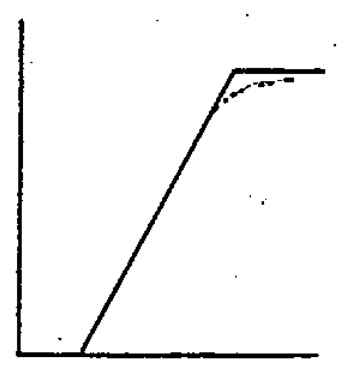
\includegraphics[width=.15\linewidth]{figs/rate1.png} &
  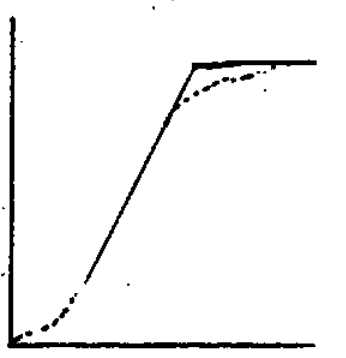
\includegraphics[width=.15\linewidth]{figs/rate2.png} &
  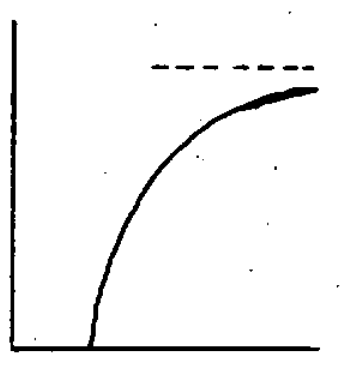
\includegraphics[width=.15\linewidth]{figs/rate3.png} &
  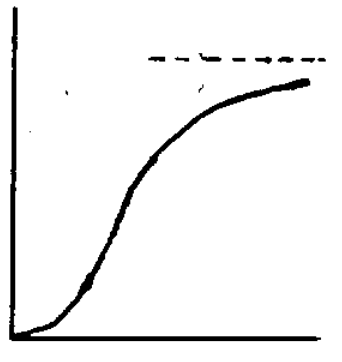
\includegraphics[width=.15\linewidth]{figs/rate4.png} \\
 & \multicolumn{4}{c}{Time in Days} \\
 & Figure 1 & Figure 2 & Figure 3 & Figure 4 \\
\end{tabular}
\end{table}

Figure 2 is like Figure 1 except that there is no induction period. Germination
starts in the first or second day. In the early stages the rate of germination is slowed
down by a deficiencies of water and oxygen in the embryo so that in the first few days
the overall rate depends not only on the rate of the chemical process, but also on the
rates of diffusion of water and oxygen through the seed coat. Within several days the
diffusion rate is no longer a factor, and the linear plot develops. Figure 2 is typical of
many common garden annuals and vegetables. The curve is like an S-shaped curve
at the beginning and at the end and can be mistaken for a true S-shaped curve.

Figures 3 and 4 are analogous to Figures 1 and 2 except that the plot is
rounded curve and of the type where in each time period, a day for example, a
constant fraction of the remaining sample germinates. This type of curve is that of a
\textit{first order} rate process, and the rate is conveniently expressed as the halftime, the
time for half of the seeds to germinate. Thus a half time or half life of five days would
mean that half of the seeds germinated in five days. This first order type of rate should
be familiar because it is the rate law for radioactive decomposition.

Even in the species that required light for germination (Chapter 11),
germinations often followed zero or first order rate laws because of the exact timings
and constant intensity of the light. Even where precise data were not recorded, it was
still possible to record induction times and the range of days or weeks over which 80-
90\% of the germination look place. Thus major changes in rates and induction time
could still be detected. These rates of germination and induction times as well as
other features of the germination have taxonomic significance and serve to
characterize taxa just as much as gross morphology, it was possible in afew examples
to detect two kinds of seeds in the sample by showing that the rate plot was a
composite of two separate rates (see Chapter 19).

Three important generalizations emerged from the rate data. \textit{First} was the
prevalence of induction periods. \textit{Second} was the extremely large changes in rates
with temperature which-were found for the reactions involving conditioning of the
seeds (see Chapter 6). \textit{Third} was the numerous examples of chemical processes that
increased in rate as the temperature was lowered (negative temperature coefficients).

The induction periods shown in Figures 1 and 3 are interpreted as chemical
time clocks involving destruction of germination inhibitors. The phenomenon of an
induction period followed by an \textit{abrupt onset} of germination (or any chemical reaction)
is diagnostic for a chemical clock reaction and the destruction of an inhibitor. It is
unlikely that the patterns in Figures 1 an 3 can be due to delays in diffusion of water
and oxygen through the seed coat, formation of germination promoters, or time
required for an embryo to grow. All of these would lead to a \textit{gradual onset} of
germination.

It might help in understanding chemical time clocks to give an example from
everyday life. Rubber bands can sit in a drawer for a year or more without any
apparent change in outward appearance or any change in their elasticity. One day
cracks start to develop and the rubber band is soon easily ruptured and ultimately
crumbles. The explanation is that raw rubber is rapidly oxidized by oxygen in air in a
complex chain reaction which results in cleavage of the polymeric chains and
crumbling of the rubber to a powder. In the manufacture of rubber \textit{chemical inhibitors}
are introduced into the rubber which block the chain reaction and preserve the rubber.
Ultimately these chemical inhibitors are used up whereupon the oxidative degradation
of the rubber abruptly begins and proceeds rapidly.

It may seem surprising to persons outside the field of physical organic chemistry
that chemical processes of multistep and complex nature can still follow simple rate
laws such as those of a zero order or first order process. The reason has been
understood for some years in physical organic chemistry in terms of a rate determining
(r.d.) step. Generally in a process consisting of a number of steps, one step will the the
slowest. Not only will it limit the rate of the overall process, but it will dictate the rate
law.

One might wonder why seeds that appear to be identical germinate over a
period of time and not all at once. The same question arises for radioactive
disintegration and in fact all chemical processes. It was one of the great triumphs of
science when Boltzmann worked out the theory of this (Boltzmann statistics). The
answer using seeds as an example is that germination requires a particular
conformation of the molecular motion and a particular concentration of energies. The
chance of achieving this for any seed at any moment is statistically determined. To
add a brief personal note, the Noble Laureate George Uhlenbeck gave a course at the
University of Michigan in which he traced the course of Boltzmann's life and the
development of his theories. My wife Virginia was taking the course so I sat in. It was
a wonderful experience, and it gave an invaluable insight into this field.
Incidentally for young people starting out in any career. Take time to broaden
your viewpoints by attending lectures in areas outside of your own. Considerable
selectivity must be exercised to avoid wasting time hearing endless garbage, but the
rewards can be great. It is the cross fertilization of fields that leads to innovation.

